%This is my super simple Real Analysis Homework template

\documentclass{article}

%% Language and font encodings
\usepackage[T1,T8K,T8M]{fontenc}
\usepackage[utf8]{inputenc}
\usepackage[english,georgian]{babel}

\usepackage{amsmath}
\usepackage{graphicx}
\usepackage[colorinlistoftodos]{todonotes}
\usepackage[colorlinks=true, allcolors=blue]{hyperref}
\usepackage{float}
\usepackage{enumerate}
\usepackage{subfig}
\usepackage{gensymb}

\begin{document}
[ჰიდროდინამიკა] \href{https://www.physolymp.spb.ru/index.php/archive/2003/245}{[წყარო]} \href{https://www.physolymp.spb.ru/index.php/archive/2003/240}{[ამოხსნა]} \\
ვერტიკალურ ჭურჭელში კვეთებით $S_1$ და $S_2$ $(S_1=9S_2)$ არის მოთავსებული ორი უმასო დგუში. დგუშებს შორის სივრცე შევსებულია წყლით. ჭურჭლის ბოლოები ღია ატმოსფეროშია. ზემო დგუშზე მიბმულია $k$ სიხისტის ზამბარა, ხოლო მეორე ქვემოთ დგუშზე $m$ მასის ტვირთი. საწყისს მომენტში ზამბარა დაუჭიმავია და დგუშები დამაგრებულია. დგუშებს შორის მანძილია $h_0$. განსაზღვრეთ რამდენით დაიწევს ზედა დგუში თუ ორივე დგუშს ხელს გავუშვებთ?
	\begin{figure}[H]
		\centering
		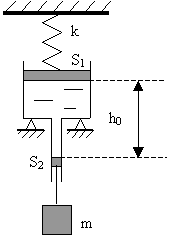
\includegraphics[width=0.2\columnwidth]{images/th07p_03_5}
		\caption{th07p0305.}
		\label{fig:th07p_03_5}
	\end{figure}

\end{document}